\section{Constructions at \Fiii{}: real multiplication on K3 surfaces}\label{sec:f3prime}

\subsection{Where the first class is}

Let $S$ be a projective K3 surface, $T=T(S)_{\QQ}$ and $E=\End_{\Hdg}T$. The Hodge classes of $S\times S$ are $H^{0}\otimes H^{4}$, $H^{4}\otimes H^{0}$ and $\End_{\Hdg}H^{2}(S)=\End(\NS_{\QQ})\oplus E$, since $T$ is irreducible with no class of type $(1,1)$ and $\Hom_{\Hdg}(T,\NS_{\QQ})=0$. The first two pieces and $\End(\NS_{\QQ})$ are spanned by products of divisor classes. So the Hodge conjecture for $S\times S$ is the algebraicity of $E$, and by Proposition~\ref{prop:abpart} the same classes decide \Fiii{} for $S\times S$ once $T$ is not reached from abelian varieties. When $E$ is a CM field it is spanned by its elements of norm one, which are Hodge isometries of $T$ and algebraic by Buskin's theorem \cite{Bus19}; see \cite[Rem.~2.16]{Var23}. When $E$ is totally real, the Rosati involution is the identity on it \cite{Zar83}, every $e\in E$ is self-adjoint for the intersection form $q$, and $q(ex,ey)=q(e^{2}x,y)$. The first class is a real multiplication.

\subsection{Chains of correspondences}

\begin{lemma}\label{lem:dominant}
Let $f\colon S\dashrightarrow S'$ be a dominant rational map of K3 surfaces of degree $d$ and $\Gamma_{f}$ the closure of its graph. Then $f_{*}=\Gamma_{f*}$ and $f^{*}=\Gamma_{f*}^{t}$ are morphisms of Hodge structures, $f^{*}$ maps $T(S')_{\QQ}$ isomorphically onto $T(S)_{\QQ}$ with $q_{S}(f^{*}a,f^{*}b)=d\,q_{S'}(a,b)$, and $f_{*}=d\,(f^{*})^{-1}$ on $T(S)_{\QQ}$.
\end{lemma}

\begin{proof}
The graph is an algebraic cycle, so both maps are induced by algebraic classes and are morphisms of Hodge structures. Pull-back of a nowhere vanishing $2$-form is a nonzero $2$-form, so $f^{*}(T(S')_{\QQ})$ is a sub-Hodge structure of $H^{2}(S)$ that meets $H^{2,0}(S)$; the smallest sub-Hodge structure of $H^{2}(S)$ containing $H^{2,0}$ is $T(S)_{\QQ}$, so $f^{*}T(S')_{\QQ}\supseteq T(S)_{\QQ}$, and since $T(S')_{\QQ}$ is irreducible and $f^{*}$ is injective on it ($f_{*}f^{*}=d$), equality of dimensions gives $f^{*}T(S')_{\QQ}=T(S)_{\QQ}$. The projection formula gives $q_{S}(f^{*}a,f^{*}b)=q_{S'}(f_{*}f^{*}a,b)=d\,q_{S'}(a,b)$ and $f_{*}f^{*}=d$.
\end{proof}

\begin{lemma}\label{lem:isometry}
A Hodge isometry $\varphi\colon T(S)_{\QQ}\to T(S')_{\QQ}$ is induced by an algebraic class on $S\times S'$.
\end{lemma}

\begin{proof}
The spaces $\NS(S)_{\QQ}$ and $\NS(S')_{\QQ}$ are the orthogonal complements of $T(S)_{\QQ}$ and $T(S')_{\QQ}$ in the two copies of $\Lambda_{\QQ}$, isometric to each other through $\varphi$; by Witt's cancellation theorem the complements are isometric, so $\varphi$ extends to a Hodge isometry $H^{2}(S)\to H^{2}(S')$, which is algebraic by Buskin's theorem \cite{Bus19} (see \cite[Thm.~0.1]{Huy19}). The projector of $H^{2}(S)$ onto $T(S)_{\QQ}$ along $\NS(S)_{\QQ}$ is algebraic, being $1$ minus the projector onto $\NS$, which is a sum $\sum_{i,j}c_{ij}\,D_{i}\otimes D_{j}$ over a basis of divisor classes with $(c_{ij})$ the inverse Gram matrix; composing gives $\varphi$ on $T$ and zero on $\NS$.
\end{proof}

\begin{theorem}[Chains]\label{thm:chain}
Let $S$ be a projective K3 surface with $E$ totally real and $e\in E$ with $e^{2}=n\in\QQ_{>0}$. Suppose there are projective K3 surfaces $S=S_{0},S_{1},\dots,S_{r}$ and, for each $i$, either a dominant rational map $S_{i-1}\dashrightarrow S_{i}$ of degree $n_{i}$, a dominant rational map $S_{i}\dashrightarrow S_{i-1}$ of degree $n_{i}$, or a Hodge isometry $T(S_{i-1})_{\QQ}\cong T(S_{i})_{\QQ}$ (and then $n_{i}=1$), such that
\[
\prod_{i}n_{i}^{\pm1}\equiv n\pmod{\QQ^{\times2}},
\]
the sign being $+$ for maps leaving $S_{i-1}$ and $-$ for maps arriving at it. Then $e$ is algebraic on $S\times S$.
\end{theorem}

\begin{proof}
Composing along the chain the maps $f_{*}$ for maps leaving $S_{i-1}$, $f^{*}$ for maps arriving, and the classes of Lemma~\ref{lem:isometry} for the isometries, gives an algebraic isomorphism $\phi\colon T(S_{r})_{\QQ}\to T(S)_{\QQ}$ of Hodge structures with $q_{S}(\phi a,\phi b)=\mu\,q_{S_{r}}(a,b)$, where $\mu=\prod n_{i}^{\pm1}$ by Lemma~\ref{lem:dominant} (a map leaving contributes $f_{*}=n_{i}(f^{*})^{-1}$, of multiplier $n_{i}$; a map arriving contributes $f^{*}$, of multiplier $n_{i}$ in the other direction, that is $n_{i}^{-1}$ for the composite in the direction of $\phi$). Write $\mu=nc^{2}$ with $c\in\QQ^{\times}$. Since $e$ is self-adjoint with $e^{2}=n$, it is a Hodge similarity of $T(S)_{\QQ}$ of multiplier $n$. So $\psi=(c^{-1}\phi)^{-1}\circ e\colon T(S)_{\QQ}\to T(S_{r})_{\QQ}$ is a Hodge isometry, algebraic by Lemma~\ref{lem:isometry}, and $e=(c^{-1}\phi)\circ\psi$ is a composite of algebraic correspondences, hence algebraic on $S\times S$.
\end{proof}

The case $r=1$ with $S\dashrightarrow S_{1}$ the quotient by a symplectic automorphism of prime order $p$ is Varesco's theorem \cite[Thm.~2.1]{Var23}, which gives $e=\sqrt p$ and is used for $p=2,3$. What a chain adds is a composite multiplier.

\subsection{Real multiplication by $\QQ(\sqrt6)$}

A symplectic automorphism of finite order on a K3 surface acts trivially on $T(S)$, its quotient has a K3 resolution $Y$ \cite{Nik80}, and $T(Y)_{\QQ}\cong T(S)_{\QQ}(1/\mathrm{ord})$ by Lemma~\ref{lem:dominant}. The invariant lattice of a symplectic involution is $U^{3}\oplus E_{8}(-2)$, and a K3 surface has a symplectic involution exactly when $E_{8}(-2)$ embeds primitively in its N\'eron--Severi lattice \cite{Mor84,vGS07}. The invariant lattice of a symplectic automorphism of order three is $U\oplus U(3)^{2}\oplus A_{2}^{2}$, and such an automorphism exists exactly when the Coxeter--Todd lattice $K_{12}(-2)$ embeds primitively in the N\'eron--Severi lattice \cite[Thm.~4.1]{GS07}. Put
\[
V_{2}=\bigl(U^{3}\oplus E_{8}(-2)\bigr)_{\QQ},\qquad V_{3}=\bigl(U\oplus U(3)^{2}\oplus A_{2}^{2}\bigr)_{\QQ},
\]
of ranks $14$ and $10$ and signatures $(3,11)$ and $(3,7)$; over $\QQ$, $U(3)\cong U$ and $E_{8}(-2)\cong\langle-1\rangle^{8}\cong\langle-2\rangle^{8}$. Varesco \cite[Props.~2.5 and 2.11]{Var23} shows that a projective K3 surface whose transcendental space embeds isometrically in $V_{2}$ (resp.\ $V_{3}$) is Hodge isometric to one with a symplectic involution (resp.\ a symplectic automorphism of order three).

\begin{lemma}[Embedding criterion]\label{lem:embed}
Let $W$ and $V$ be rational quadratic spaces with $\mathrm{rk}\,V-\mathrm{rk}\,W\ge3$. Then $W$ embeds isometrically in $V$ if and only if the signature of $V$ dominates that of $W$ in both signs. In that case a complement $W'$ exists with $V\cong W\oplus W'$.
\end{lemma}

\begin{proof}
Necessity is clear. For sufficiency put $k=\mathrm{rk}\,V-\mathrm{rk}\,W\ge3$ and let $(s_{+},s_{-})$ be the difference of signatures, $s_{+}+s_{-}=k$. A quadratic space $W'$ of rank $k$ and signature $(s_{+},s_{-})$ with prescribed discriminant $d'=d(V)d(W)$ and prescribed Hasse invariants $\varepsilon_{p}'$ exists provided the $\varepsilon'_{p}$ equal $1$ for almost all $p$, $\prod_{p\le\infty}\varepsilon'_{p}=1$, and $\varepsilon'_{\infty}$, $d'$ match the signature \cite[Chap.~IV, Prop.~7]{Ser73}, with no further condition when $k\ge3$. Take $\varepsilon'_{p}=\varepsilon_{p}(V)\varepsilon_{p}(W)(d(W),d')_{p}$, the value forced by the formula $\varepsilon_{p}(W\oplus W')=\varepsilon_{p}(W)\varepsilon_{p}(W')(d(W),d(W'))_{p}$. The product formula for these holds because it holds for $V$, for $W$ and for the Hilbert symbol. Then $W\oplus W'$ and $V$ have the same rank, signature, discriminant and Hasse invariants at every place, so they are isometric by the Hasse--Minkowski theorem \cite[Chap.~IV, Thm.~9]{Ser73}, and $W$ embeds in $V$.
\end{proof}

\begin{theorem}[Two-dimensional families with algebraic real multiplication by $\QQ(\sqrt6)$]\label{thm:sqrt6}
Let $S$ be a projective K3 surface with $\QQ(\sqrt6)\subseteq E$ whose transcendental space $T=T(S)_{\QQ}$ embeds isometrically in $V_{3}$.
\begin{enumerate}[label=\textup{(\roman*)},leftmargin=2.4em,itemsep=2pt]
\item $\sqrt6\in E$ is algebraic on $S\times S$.
\item The Hodge conjecture, and \Fiii{}, hold for $S\times S$ and for the Hilbert square $S^{[2]}$.
\item Such surfaces exist in two-dimensional families, whose very general member has $\mathrm{rk}\,T=8$ and $E=\QQ(\sqrt6)$ exactly. One such family is the one whose transcendental space is $E^{4}$ with the trace form of $q_{E}=\langle-2,-2,-2+\sqrt6,-1+\sqrt6\rangle$ over $E=\QQ(\sqrt6)$.
\end{enumerate}
\end{theorem}

\begin{proof}
(i) By \cite[Prop.~2.11]{Var23} $S$ is Hodge isometric to a K3 surface $S'$ with a symplectic automorphism $\sigma$ of order three, and by Lemma~\ref{lem:isometry} the isometry is algebraic, so we may replace $S$ by $S'$. Let $Y$ be the minimal resolution of $S'/\sigma$ and $f_{1}\colon S'\dashrightarrow Y$ the quotient map, of degree three, so that $T(Y)_{\QQ}\cong T(1/3)$, of rank $\mathrm{rk}\,T\le8$ and signature $(2,\mathrm{rk}\,T-2)$: the rank is at most $8$ because $T$ embeds in $V_{3}$ of rank $10$ and signature $(3,7)$ with a complement that must contain the remaining positive direction, so the complement has rank at least two. Now $T(Y)_{\QQ}$ has rank at most $8$ and signature dominated by $(3,11)$, and $14-8\ge3$, so by Lemma~\ref{lem:embed} it embeds in $V_{2}$. By \cite[Prop.~2.5]{Var23} $Y$ is Hodge isometric to a K3 surface $Y'$ with a symplectic involution $\iota$; let $Z$ be the resolution of $Y'/\iota$ and $f_{2}\colon Y'\dashrightarrow Z$ the quotient, of degree two. The chain $S'\dashrightarrow Y\cong Y'\dashrightarrow Z$ has multiplier $3\cdot1\cdot2=6$, and Theorem~\ref{thm:chain} applies to $e=\sqrt6$ (Fig.~\ref{fig:chain}).

(ii) By the first paragraph of this section it remains to make $E$ algebraic. $E$ contains $\QQ(\sqrt6)$, and either $E=\QQ(\sqrt6)$ or $E$ is a CM field: a totally real $E$ has $\dim_{E}T\ge3$, because the complex line $H^{2,0}$ lies in one eigenspace $T_{\sigma}\otimes\CC$ and $\overline{H^{2,0}}$ in the same one, so that $T_{\sigma}\otimes\RR$ has signature $(2,\ast)$ and $\dim_{E}T\ge3$ follows from $q$ being negative definite on the other eigenspaces together with $T\otimes\RR$ having exactly two positive directions; and $[E:\QQ]\cdot\dim_{E}T=\mathrm{rk}\,T\le8$ then forces $[E:\QQ]\le2$. If $E=\QQ(\sqrt6)$, (i) suffices. If $E$ is CM, it is spanned by its norm-one elements, Hodge isometries, algebraic by Buskin's theorem. So every Hodge class on $S\times S$ is algebraic, and \Fiii{} follows. For $S^{[2]}$ the Chow motive is a direct summand of twists of $h(S\times S)$, $h(S)$ and $\mathbf{1}$ \cite{dCM02}, so every Hodge class on $S^{[2]}$ is the image under an algebraic correspondence of a Hodge class on $S\times S$ or $S$, and both statements follow.

(iii) Let $E=\QQ(\sqrt6)$ with real embeddings $\sigma_{1}$, $\sigma_{2}$ ($\sqrt6\mapsto\pm\sqrt6$), and let $q_{E}=\langle a_{1},a_{2},a_{3},a_{4}\rangle$ with $a_{1},a_{2}$ negative at both places and $a_{3},a_{4}$ positive at $\sigma_{1}$, negative at $\sigma_{2}$. The $\QQ$-space $T=E^{4}$ with the form $\Tr_{E/\QQ}\circ q_{E}$ has rank $8$ and signature $(2,2)+(0,4)=(2,6)$, and multiplication by $\sqrt6$ is self-adjoint of square $6$. For $q_{E}=\langle-2,-2,-2+\sqrt6,-1+\sqrt6\rangle$ one computes $d(T)=10$, $\varepsilon_{2}=1$, $\varepsilon_{3}=-1$, $\varepsilon_{5}=1$ and $\varepsilon_{p}=1$ otherwise, while $V_{3}$ has $d=-1$, $\varepsilon_{2}=1$, $\varepsilon_{3}=-1$, $\varepsilon_{5}=1$; and $T\oplus\langle1,-10\rangle$ has the invariants of $V_{3}$ at every place, so $V_{3}\cong T\oplus\langle1,-10\rangle$ by Hasse--Minkowski, with a complement containing a positive vector (Table~\ref{tab:invariants}; the Hilbert symbols are recomputed in the programs of Appendix~\ref{app:checks}). Embed $V_{3}$ in $\Lambda_{\QQ}$ as the invariant lattice of an order-three symplectic action, with orthogonal complement $K_{12}(-2)$, and let $N\subseteq\Lambda$ be the primitive sublattice with $N_{\QQ}=T^{\perp}$; it contains $K_{12}(-2)$ primitively and a positive class. The Hodge structures of K3 type on $T$ for which $\sqrt6$ is a Hodge endomorphism are the periods $\omega\in\PP(T_{\sigma_{1}}\otimes\CC)$ with $q(\omega)=0$, $q(\omega,\bar\omega)>0$, where $T_{\sigma_{1}}$ is the $\sigma_{1}$-eigenspace, of signature $(2,2)$; this is a domain of dimension two \cite[Prop.~2.3]{Var23}. For each such $\omega$ the surjectivity of the period map gives a K3 surface $S_{\omega}$ with $T(S_{\omega})_{\QQ}\subseteq T$, projective because $N$ contains a positive class, carrying an order-three symplectic automorphism because $K_{12}(-2)\subseteq N$ primitively. For $\omega$ outside a countable union of proper closed analytic subsets, $T(S_{\omega})_{\QQ}=T$ and $E=\QQ(\sqrt6)$, by the argument of \cite[Thm.~22.9]{BMB26}, which needs only $\dim_{E}T\ge3$.
\end{proof}

\begin{table}[t]
\centering
\caption{Rational invariants used in Theorem~\ref{thm:sqrt6}(iii). Hasse invariants are $+1$ at every prime not shown.}
\label{tab:invariants}
\begin{ruledtabular}
\begin{tabular}{lcccccc}
space & rank & signature & $d$ & $\varepsilon_{2}$ & $\varepsilon_{3}$ & $\varepsilon_{5}$ \\
\colrule
$T=\Tr_{E/\QQ}q_{E}$ & 8 & $(2,6)$ & $10$ & $+1$ & $-1$ & $+1$ \\
$\langle1,-10\rangle$ & 2 & $(1,1)$ & $-10$ & $+1$ & $+1$ & $+1$ \\
$T\oplus\langle1,-10\rangle$ & 10 & $(3,7)$ & $-1$ & $+1$ & $-1$ & $+1$ \\
$V_{3}$ & 10 & $(3,7)$ & $-1$ & $+1$ & $-1$ & $+1$ \\
$V_{2}$ & 14 & $(3,11)$ & $-1$ & $-1$ & $+1$ & $+1$ \\
\end{tabular}
\end{ruledtabular}
\end{table}

\begin{figure}[t]
\centering
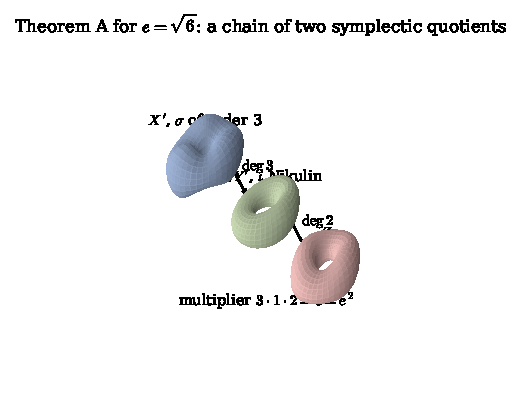
\includegraphics[width=0.95\columnwidth]{figures/fig_chain}
\caption{The chain of Theorem~\ref{thm:sqrt6}: the quotient of $S'$ by a symplectic automorphism of order three, a Hodge isometry (algebraic by Buskin), and the quotient of $Y'$ by a Nikulin involution. The multipliers compose to $6$.}
\label{fig:chain}
\end{figure}

Varesco's families have $E=\QQ(\sqrt2)$ or $\QQ(\sqrt3)$ \cite[Thms.~2.9, 2.15]{Var23}; van Geemen and Sch\"utt obtain $\sqrt2$, $\sqrt3$, $\sqrt7$ from rational self-maps of elliptic K3 surfaces \cite[\S\S6--7]{vGS25}; Bayer-Fluckiger, van Geemen and Sch\"utt prove that families with real multiplication by any totally real $E$ with $[E:\QQ]\dim_{E}T\le21$ exist, without algebraicity \cite{BvGS24}. The lattice condition of Theorem~\ref{thm:sqrt6} is a genuine restriction: among the $165$ sign-admissible diagonal forms $q_{E}$ with small coefficients, $98$ embed in $V_{3}$ and $67$ do not (Appendix~\ref{app:checks}).

\subsection{Isogenies of elliptic surfaces}\label{ssec:fricke}

Varesco's quotients and the chains of Theorem~\ref{thm:chain} produce the square roots of the orders of symplectic automorphisms, $2$ and $3$, and their products. A different source of similarities is a rational self-map of a K3 surface, and the self-maps that exist in families come from isogenies of elliptic fibrations: van Geemen and Sch\"utt obtain $\sqrt2$ and $\sqrt3$ from isogenies of degree $2$ and $3$ in this way, and for degrees $5$ and $7$ they give one surface each \cite[\S\S6--7]{vGS25}. We show that the degrees $5$ and $7$ also come in families.

Let $N\in\{5,7\}$ and write $N^{k}$ for $125$ when $N=5$ and $49$ when $N=7$. The modular curve $X_{0}(N)$ is rational, with Fricke's coordinate $t$ in which the involution $(E,C)\mapsto(E/C,E[N]/C)$ is $w(t)=N^{k}/t$ \cite[\S7.6]{vGS25}. The universal curve with a cyclic subgroup $C_{t}$ of order $N$ over $\PP^{1}_{t}$ is
\begin{equation}\label{eq:fricke}
\mathcal{E}_{t}\colon\ y^{2}=x^{3}-27c_{4}(t)\,x-54c_{6}(t),
\end{equation}
with, for $N=7$,
\begin{align*}
c_{4}&=(t^{2}+13t+49)(t^{2}+5t+1),\\
c_{6}&=(t^{2}+13t+49)(t^{4}+14t^{3}+63t^{2}+70t-7),
\end{align*}
and for $N=5$,
\begin{align*}
c_{4}&=(t^{2}+10t+5)(t^{2}+22t+125),\\
c_{6}&=(t^{2}+4t-1)(t^{2}+22t+125)^{2}.
\end{align*}
The discriminant is $1728\,t\,(t^{2}+13t+49)^{2}$ for $N=7$ and $1728\,t\,(t^{2}+22t+125)^{3}$ for $N=5$, of degree $5$ and $7$. So the relatively minimal model $R_{N}$ of \eqref{eq:fricke} over $\PP^{1}_{t}$ is a rational elliptic surface with fibres of type $\mathrm{I}_{1}$ at $t=0$, $\mathrm{I}_{N}$ at $t=\infty$, and at the two roots $e_{1},e_{2}$ of the quadratic factor, where $c_{4}$ vanishes, of type $\mathrm{II}$ for $N=7$ and $\mathrm{III}$ for $N=5$; the Euler numbers add up to $1+N+2\cdot2=12$ and $1+N+2\cdot3=12$. The roots satisfy $e_{1}e_{2}=N^{k}$, so $w$ exchanges them and exchanges $0$ with $\infty$.

\begin{lemma}[The Fricke isogeny over the function field]\label{lem:fricke}
$\mathcal{E}_{t}/C_{t}\cong\mathcal{E}_{w(t)}$ over $\CC(t)$.
\end{lemma}

\begin{proof}
The two curves have the same $j$-invariant, because $w$ is the Fricke involution of $X_{0}(N)$. Two elliptic curves over $\CC(t)$ with the same non-constant $j$-invariant differ by a quadratic twist $\chi\in\CC(t)^{\times}/\CC(t)^{\times2}$, and a twist ramified at a point of $\PP^{1}$ changes the Kodaira type of the fibre there, exchanging $\mathrm{I}_{n}$ with $\mathrm{I}_{n}^{*}$, $\mathrm{II}$ with $\mathrm{IV}^{*}$ and $\mathrm{III}$ with $\mathrm{III}^{*}$. So it suffices to show that $\mathcal{E}_{t}/C_{t}$ has the same fibre types as $\mathcal{E}_{w(t)}$, which are $\mathrm{I}_{N}$ at $0$, $\mathrm{I}_{1}$ at $\infty$ and $\mathrm{II}$ or $\mathrm{III}$ at $e_{1},e_{2}$: then $\chi$ is unramified on $\PP^{1}$, hence constant, hence trivial over $\CC$.

At $t=0$ the fibre of $\mathcal{E}$ is $\mathrm{I}_{1}$, the Tate curve $\mathbb{G}_{m}/q^{\ZZ}$ over $\CC((t))$, whose only cyclic subgroup of order $N$ rational over $\CC((t))$ is $\mu_{N}$; the quotient $\mathbb{G}_{m}/q^{N\ZZ}$ is $\mathrm{I}_{N}$. At $e_{i}$ the local monodromy $M\in\SL_{2}(\ZZ)$ of $\mathcal{E}$ has order $6$ or $4$ and irreducible characteristic polynomial; the isogeny is given on the period lattices by a matrix $A\in M_{2}(\ZZ)$ with $\det A=N$, and the monodromy of the quotient is $M'=AMA^{-1}$. The $\SL_{2}(\ZZ)$-classes with this characteristic polynomial are those of $M$ and $M^{-1}$, which are the types $\mathrm{II}$ and $\mathrm{II}^{*}$, or $\mathrm{III}$ and $\mathrm{III}^{*}$. If $M'=gM^{-1}g^{-1}$ with $g\in\SL_{2}(\ZZ)$, then $B=g^{-1}A$ conjugates $M$ to $M^{-1}$. All rational matrices doing so form the coset $B_{0}\,\QQ(M)^{\times}$, where $B_{0}=\bigl(\begin{smallmatrix}0&1\\1&0\end{smallmatrix}\bigr)$ for $M=\bigl(\begin{smallmatrix}0&-1\\1&\mathrm{tr}M\end{smallmatrix}\bigr)$ has determinant $-1$ and the elements of the imaginary quadratic field $\QQ(M)$ have positive norm; so $\det B<0$, against $\det B=N$. Hence the quotient has the type of $M$ at $e_{1},e_{2}$. At $\infty$ the $j$-invariant of the quotient has a simple pole, so the fibre is $\mathrm{I}_{1}$ or $\mathrm{I}_{1}^{*}$, and the Euler numbers of the other fibres add up to $11$; since the total is $12$ the fibre is $\mathrm{I}_{1}$.
\end{proof}

For $p\ne q$ in $\PP^{1}_{t}$ let $u_{p,q}=(t-p)(t-q)$, and let $X_{p,q}$ be the elliptic K3 surface whose generic fibre is the quadratic twist $\mathcal{E}_{t}\otimes u_{p,q}$: the twist multiplies $c_{4}$ by $u^{2}$ and $c_{6}$ by $u^{3}$, giving Weierstrass coefficients of degrees $8$ and $12$, and adds two fibres of type $\mathrm{I}_{0}^{*}$ at $p$ and $q$ when these are not among $0,\infty,e_{1},e_{2}$. For a double cover $\psi\colon\PP^{1}_{s}\to\PP^{1}_{t}$ let $X_{\psi}$ be the relatively minimal model of $\psi^{*}\mathcal{E}$.

\begin{lemma}\label{lem:twists}
\leavevmode
\begin{enumerate}[label=\textup{(\roman*)},leftmargin=2.4em,itemsep=2pt]
\item $X_{p,q}$ has Picard number at least $16$: its Néron--Severi lattice contains $U\oplus A_{6}\oplus D_{4}^{2}$ for $N=7$ and $U\oplus A_{4}\oplus A_{1}^{2}\oplus D_{4}^{2}$ for $N=5$. The same bound holds for $X_{\psi}$, whose fibres $2\,\mathrm{I}_{1}+2\,\mathrm{I}_{N}$, together with four fibres of type $\mathrm{III}$ when $N=5$, and the pulled-back Mordell--Weil group of $R_{N}$, of rank $2$, give rank at least $16$ by the Shioda--Tate formula.
\item The fibrewise isogeny by $C_{t}$ is a dominant rational map of degree $N$
\[
f\colon X_{p,q}\dashrightarrow X_{w(p),w(q)},\qquad f\colon X_{\psi}\dashrightarrow X_{w\circ\psi}.
\]
\item The deck involution of $\psi$ times $[-1]$ on the fibres is a symplectic involution $\iota$ of $X_{\psi}$, and the minimal resolution of $X_{\psi}/\iota$ is $X_{p,q}$ with $\{p,q\}$ the branch locus of $\psi$. Hence $T(X_{\psi})_{\QQ}\cong T(X_{p,q})_{\QQ}(1/2)$ as in Lemma~\ref{lem:dominant}, and the two surfaces have the same Picard number.
\end{enumerate}
\end{lemma}

\begin{proof}
(i) Shioda--Tate with the fibres listed, and for $X_{\psi}$ the Mordell--Weil rank $8-6=2$ of $R_{N}$. (ii) By Lemma~\ref{lem:fricke} the quotient of the generic fibre is $\mathcal{E}_{w(t)}\otimes u_{p,q}(t)$, and
\[
u_{p,q}(w(t))=\Bigl(\frac{N^{k}}{t}-p\Bigr)\Bigl(\frac{N^{k}}{t}-q\Bigr)=\frac{pq}{t^{2}}\,u_{w(p),w(q)}(t),
\]
a constant times a square times $u_{w(p),w(q)}$. So $\mathcal{E}_{w(t)}\otimes u_{p,q}(t)\cong\mathcal{E}_{w(t)}\otimes u_{w(p),w(q)}(w(t))$, which is the pull-back along the automorphism $w$ of the base of the generic fibre of $X_{w(p),w(q)}$; pulling back along an automorphism of the base gives an isomorphic surface. For $X_{\psi}$, $(\psi^{*}\mathcal{E})/C=\psi^{*}(\mathcal{E}/C)\cong\psi^{*}w^{*}\mathcal{E}$. (iii) The quadratic twist by the function defining the double cover is the quotient of the base change by the deck involution composed with $[-1]$ on the fibres; the involution is symplectic with eight fixed points, the $2$-torsion of the two fibres over the ramification points, and the quotient's resolution is the twist.
\end{proof}

\begin{theorem}[One-dimensional families with algebraic real multiplication by $\sqrt5$ and $\sqrt7$]\label{thm:fricke}
Let $N\in\{5,7\}$ and let $\mathfrak{A}_{N}$ be the family of surfaces $X_{p}=X_{p,N^{k}/p}$ for $p\notin\{0,\infty,e_{1},e_{2},\pm\sqrt{N^{k}}\}$, and $\mathfrak{B}_{N}$ the family of surfaces $X_{\psi}$ with $\psi$ branched over a pair $\{b,N^{k}/b\}$.
\begin{enumerate}[label=\textup{(\roman*)},leftmargin=2.4em,itemsep=2pt]
\item Every member $X$ has a dominant rational self-map $f$ of degree $N$, and $f^{*}$ is an element of $E=\End_{\Hdg}T(X)_{\QQ}$ with $f^{*}f_{*}=N$.
\item The families are not isotrivial. Their very general member has Picard number $16$, transcendental rank $6$ and $E=\QQ(\sqrt N)$, with $\sqrt N=\pm f^{*}$ algebraic on $X\times X$.
\item For every member $X$ the Hodge conjecture holds for $X\times X$, and \Fiii{} holds for $X\times X$ and for $X^{[2]}$.
\end{enumerate}
\end{theorem}

\begin{proof}
(i) $w$ exchanges $p$ and $N^{k}/p$, so Lemma~\ref{lem:twists}(ii) gives $f\colon X_{p}\dashrightarrow X_{p}$; for $\mathfrak{B}_{N}$, $w\circ\psi$ has the same branch locus as $\psi$, so $w\circ\psi=\psi\circ\sigma$ for a M\"obius transformation $\sigma$ and $X_{w\circ\psi}\cong X_{\psi}$. The correspondence of a dominant rational map preserves $\NS$ and its transpose does too, so it preserves $T=\NS^{\perp}$ and acts there as a morphism of Hodge structures, nonzero since $f^{*}\omega=\lambda\omega$ with $\lambda\ne0$; on a resolution $S$ of the graph with $p_{1}\colon S\to X$ birational and $p_{2}$ of degree $N$, both $p_{1}^{*}T$ and $p_{2}^{*}T$ are irreducible sub-Hodge structures of $H^{2}(S)$ containing its unique $(2,0)$-line, so they coincide, and $f_{*}f^{*}=p_{2*}p_{1}^{*}p_{1*}p_{2}^{*}=N$ on $T$.

(ii) The elliptic fibration of $X_{p}$ has labelled singular fibres $\mathrm{I}_{1}$ at $0$, $\mathrm{I}_{N}$ at $\infty$, $\mathrm{II}$ or $\mathrm{III}$ at $e_{1},e_{2}$ and $\mathrm{I}_{0}^{*}$ at $p$ and $N^{k}/p$. An isomorphism of elliptic fibrations induces a M\"obius transformation preserving this configuration; the transformations preserving $\{0,\infty\}$ and $\{e_{1},e_{2}\}$ are $t\mapsto\lambda t$ and $t\mapsto\lambda/t$ with $\lambda e_{1}\in\{e_{1},e_{2}\}$, and since $e_{1}+e_{2}\ne0$ and $e_{1}^{2}\ne e_{2}^{2}$ they are the identity and $w$, which preserve $\{p,N^{k}/p\}$. So $X_{p}$ and $X_{p'}$ have isomorphic fibrations only when $p'\in\{p,N^{k}/p\}$. A K3 surface has finitely many elliptic fibrations up to automorphisms \cite{Ste85}, so the map $p\mapsto[X_{p}]$ to the moduli space has finite fibres and the family is not isotrivial; by local Torelli its period map has uncountable image. A Hodge structure of K3 type on a fixed rational quadratic space with $E$ a CM field is determined by $E$, a subalgebra of the endomorphism algebra, and by an eigenline of $E\otimes\CC$, so there are countably many; the very general member is therefore not of CM type, and its $E$ is totally real. It contains $f^{*}$, and $f_{*}=N(f^{*})^{-1}$ is the adjoint of $f^{*}$, equal to $f^{*}$ since the adjoint involution is trivial on a totally real $E$; so $(f^{*})^{2}=N$ and $E\ne\QQ$. A totally real $E\ne\QQ$ has $\dim_{E}T\ge3$ \cite{vG08}, so $\mathrm{rk}\,T\ge6$; with $\rho\ge16$ this gives $\mathrm{rk}\,T=6$, $\rho=16$, $[E:\QQ]=2$ and $E=\QQ(\sqrt N)$. The same holds for $\mathfrak{B}_{N}$ by Lemma~\ref{lem:twists}(iii).

(iii) For every member $E\supseteq\QQ(\sqrt N)$ and $\mathrm{rk}\,T\le6$. If $E$ is totally real then $\dim_{E}T\ge3$ forces $E=\QQ(\sqrt N)=\QQ+\QQ f^{*}$, algebraic. Otherwise $E$ is a CM field, and every element of $E$ of norm one to its real subfield is a Hodge isometry of $T$, extended by the identity on $\NS$ to a Hodge isometry of $H^{2}(X,\QQ)$, algebraic by Buskin's theorem \cite{Bus19}. The algebraic classes form a $\QQ$-subalgebra $E'\subseteq E$ containing these elements; for $x\in E$ with $\bar x\ne x$ and $t_{1}\ne t_{2}$ in $\QQ$ it contains $(t_{i}+x)/(t_{i}+\bar x)$, hence their quotient $1+(t_{2}-t_{1})/(t_{1}+\bar x)$, hence $\bar x$; so $E'=E$. In both cases $\End_{\Hdg}H^{2}(X)=\End(\NS)\oplus E$ is algebraic, and $\Hdg^{2}(X\times X)=\End_{\Hdg}H^{2}(X)\oplus H^{0}\otimes H^{4}\oplus H^{4}\otimes H^{0}$ since $H^{1}=H^{3}=0$; the Hodge conjecture holds for $X\times X$, which gives \Fiii{} there, and passes to $X^{[2]}$ by \cite{dCM02}.
\end{proof}

\begin{figure}[t]
\centering
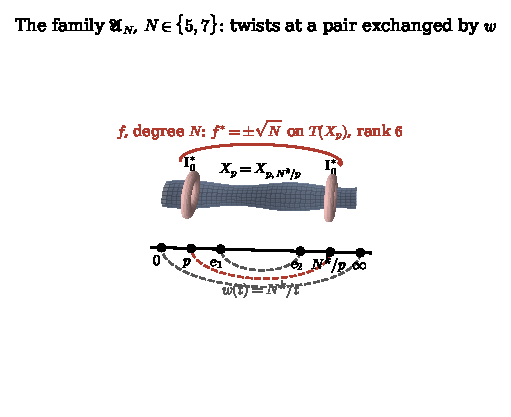
\includegraphics[width=0.95\columnwidth]{figures/fig_fricke}
\caption{The family $\mathfrak{A}_{N}$ of Theorem~\ref{thm:fricke}. Over the Fricke coordinate $t$ of $X_{0}(N)$ the involution $w(t)=N^{k}/t$ exchanges the cusps $0$, $\infty$ and the elliptic points $e_{1}$, $e_{2}$; the twist $X_{p}$ at a pair $\{p,N^{k}/p\}$ exchanged by $w$ is carried to itself by the fibrewise isogeny $f$ of degree $N$, and $f^{*}$ is the real multiplication by $\sqrt N$ on the transcendental lattice of rank six.}
\label{fig:fricke}
\end{figure}

The surface of \cite[\S7.6]{vGS25} with real multiplication by $\sqrt7$ is the twist at $\{7,-7\}$, the two fixed points of $w$, and the surface of \cite[Prop.~7.7]{vGS25} is the twist at the fixed points $\pm5\sqrt5$ for $N=5$, which has Picard number $18$ and complex multiplication. The families $\mathfrak{A}_{N}$ are the twists at the pairs exchanged by $w$; they are one-dimensional, their very general member has real and not complex multiplication, and for $N=5$ they are the first K3 surfaces of transcendental rank six with real multiplication by $\sqrt5$ that we know to carry an algebraic $\sqrt5$. The chains of Theorem~\ref{thm:chain} apply to every member: a transcendental space of rank six embeds in $V_{2}$ and $V_{3}$ with any rational scaling, so a member whose $E$ happened to contain $\sqrt{2N}$, $\sqrt{3N}$ or $\sqrt{6N}$ would have that element algebraic as well. We do not know such a member: the twist families of fixed Picard number $16$ are two-dimensional, the real multiplication loci for a fixed quadratic field on a transcendental space of rank six are one-dimensional inside a four-dimensional period domain, and the intersection has expected dimension $-1$.

\subsection{The reach of similarities}

Every correspondence used so far acts on transcendental spaces as a Hodge similarity. The next proposition says that this is not an accident of the examples but a property of every correspondence whose components are small, and it measures what a correspondence must look like to act otherwise.

\begin{proposition}[Structure of the transcendental action]\label{prop:structure}
Let $X$, $X'$ be projective K3 surfaces, $\Gamma\in\mathrm{CH}^{2}(X\times X')_{\QQ}$, and $\gamma_{T}\colon T(X)_{\QQ}\to T(X')_{\QQ}$ the map induced on transcendental spaces by composing the action of $\Gamma$ with the orthogonal projections.
\begin{enumerate}[label=\textup{(\roman*)},leftmargin=2.4em,itemsep=2pt]
\item $\gamma_{T}$ is zero or an isomorphism of Hodge structures.
\item If $\gamma_{T}\ne0$ then $a=\gamma_{T}^{\dagger}\gamma_{T}$ lies in the maximal totally real subfield of $E=\End_{\Hdg}T(X)_{\QQ}$ and is totally positive, and $\gamma_{T}$ is a similarity exactly when $a\in\QQ$.
\item Let $\Gamma$ be irreducible, $S$ a resolution of its normalisation with projections $p_{1},p_{2}$ of degrees $d_{1},d_{2}$ to $X$, $X'$. If $p_{1}^{*}T(X)_{\QQ}=p_{2}^{*}T(X')_{\QQ}$ inside $H^{2}(S,\QQ)$, then $\gamma_{T}$ is a similarity of multiplier $d_{1}d_{2}$. This holds whenever $p_{g}(S)\le1$.
\item If $\Gamma$ is irreducible and $\gamma_{T}$ is not a similarity, then $p_{1}^{*}T(X)_{\QQ}\cap p_{2}^{*}T(X')_{\QQ}=0$, so $p_{g}(S)\ge2$ and the transcendental rank of $S$ is at least twice that of $X$.
\item The $\QQ$-algebra generated by the actions on $T(X)_{\QQ}$ of all correspondences from $X$ to itself whose irreducible components either fail to dominate a factor or have $p_{g}\le1$ is the multiquadratic subfield $E_{2}\subseteq E$ generated by the square roots of the products $d_{1}d_{2}$ that occur. When $[E:\QQ]$ is odd it is $\QQ$.
\end{enumerate}
\end{proposition}

\begin{proof}
(i) $T(X)_{\QQ}$ is an irreducible Hodge structure \cite{Zar83}, and the image of $\gamma_{T}$ is a sub-Hodge structure of $H^{2}(X')$; if nonzero it contains the $(2,0)$-part, hence $T(X')_{\QQ}$, and $\gamma_{T}$ is injective by irreducibility. (ii) $a$ is a Hodge endomorphism of $T(X)$, so $a\in E$, and it is self-adjoint, so it lies in the fixed field of the adjoint involution, the maximal totally real subfield. The form $q'(\gamma x,\gamma y)=q(x,ay)$ is a polarisation of the Hodge structure $T(X)$ up to sign on each real eigenspace of $E$, and comparison with $q$ gives $\sigma(a)>0$ at every real place. A similarity of multiplier $\mu$ has $a=\mu$. (iii) Both $p_{i}^{*}T$ are irreducible sub-Hodge structures of $H^{2}(S)$ with a $(2,0)$-part; if $p_{g}(S)\le1$ they share the unique $(2,0)$-line, so they meet and coincide. When they coincide, $\gamma_{T}=p_{2*}p_{1}^{*}=d_{2}(p_{2}^{*})^{-1}p_{1}^{*}$ on $T$, so $p_{2}^{*}\gamma x=d_{2}\,p_{1}^{*}x$; since $q_{S}(p_{1}^{*}x,p_{1}^{*}y)=d_{1}q(x,y)$ and $q_{S}(p_{2}^{*}x',p_{2}^{*}y')=d_{2}q'(x',y')$, this gives $d_{2}\,q'(\gamma x,\gamma y)=q_{S}(p_{2}^{*}\gamma x,p_{2}^{*}\gamma y)=d_{2}^{2}\,q_{S}(p_{1}^{*}x,p_{1}^{*}y)=d_{1}d_{2}^{2}\,q(x,y)$, that is $q'(\gamma x,\gamma y)=d_{1}d_{2}\,q(x,y)$. (iv) If the two subspaces met they would coincide by irreducibility and (iii) would apply; so they are independent, their $(2,0)$-lines are distinct, and their sum has rank $2\,\mathrm{rk}\,T(X)$ inside the transcendental part of $H^{2}(S)$. (v) A component that does not dominate a factor acts through $\NS$ or through $H^{0}$ and $H^{4}$, hence by zero on $T$. The others act by similarities by (iii), a composite of similarities returning to $X$ is an element $\Phi\in E$ with $\Phi^{\dagger}\Phi\in\QQ$, and for totally real $E$ this is $\Phi^{2}\in\QQ$; such elements generate $E_{2}$. For a CM field $E$ the elements with $\Phi^{\dagger}\Phi\in\QQ$ are the $\QQ^{\times}$-multiples of the norm-one elements, which generate $E$, so the statement is about the totally real case, which is the one that matters for \Fiii{}. An odd-degree field has $E_{2}=\QQ$.
\end{proof}

The correspondences of Lemmas~\ref{lem:dominant} and \ref{lem:isometry}, the Fourier--Mukai kernels between a K3 surface and its moduli spaces of sheaves, the rational Hodge isometries of hyper-K\"ahler varieties of K3$^{[n]}$ type \cite{Mar24}, the Fricke isogenies of Theorem~\ref{thm:fricke} and all their composites fall under (iii) or (v). A correspondence that realises an element of a cubic field must therefore have a component whose resolution has $p_{g}\ge2$ and transcendental rank at least twice that of the surface. Such correspondences exist, and the only ones we know come from finite groups.

\begin{proposition}[Hecke correspondences]\label{prop:hecke}
Let $Z$ be a smooth projective surface with an action of a finite group $G$, $H\le G$ a subgroup, and $X$ a smooth projective surface with $p_{g}(X)=1$ birational to $Z/H$; write $\pi\colon Z\dashrightarrow X$.
\begin{enumerate}[label=\textup{(\roman*)},leftmargin=2.4em,itemsep=2pt]
\item For $g\in G$ the correspondence $\Gamma_{g}=(\pi\times\pi)_{*}[\text{graph of }g]$ acts on $H^{2}(X,\QQ)$ as the Hecke operator of the double coset $HgH$, and these operators span a $\QQ$-algebra isomorphic to a quotient of $\End_{G}\QQ[G/H]$ acting by Hodge endomorphisms.
\item Exactly one simple factor of this algebra acts nontrivially on $H^{2,0}(X)$; it is a field, it preserves $T(X)_{\QQ}$, and it embeds into $E$ by algebraic correspondences. If $H^{2,0}(Z)^{G}=0$ this factor is not the one on which $G$ acts trivially.
\item Every field obtained in this way is abelian over $\QQ$. In particular a totally real cubic field $F$ whose Galois closure has group $S_{3}$ is realised by no correspondence built from a finite group acting on a cover of $X$.
\end{enumerate}
\end{proposition}

\begin{proof}
(i) Let $\tilde Z\to Z$ be an equivariant resolution and $\pi\colon\tilde Z\to X$ the quotient by $H$ followed by the resolution; then $\pi_{*}\pi^{*}=|H|$ and $\pi_{*}h^{*}=\pi_{*}$ for $h\in H$, so $\Gamma_{g}$ acts as $\pi_{*}g^{*}\pi^{*}=(\pi^{*})^{-1}\circ\sum_{h\in HgH/H}h^{*}\circ\pi^{*}$ on $H^{2}(X,\QQ)=H^{2}(\tilde Z,\QQ)^{H}$, the Hecke operator of $HgH$. The Hecke operators of $(G,H)$ span $\End_{G}\QQ[G/H]$, a semisimple algebra, and the action on $H^{2}(\tilde Z,\QQ)^{H}$ factors through it. (ii) The idempotents of the simple factors are rational combinations of Hecke operators, so they are Hodge endomorphisms of $H^{2}(X)$; they sum to $1$ and act on the line $H^{2,0}(X)$ by $0$ or $1$, so exactly one of them, $e_{V}$, acts as $1$. A simple factor with nonzero image in the commutative ring $\End_{\Hdg}H^{2,0}(X)=\CC$ through a ring homomorphism to a field is commutative, hence a field $\mathcal{H}_{V}$. For $f\in\mathcal{H}_{V}$, $f(T(X)_{\QQ})$ is a sub-Hodge structure of the transcendental part of $H^{2}(X)$; if $f\omega\ne0$ it contains $\omega$, hence $T(X)_{\QQ}$, and if $f\omega=0$ it has no $(2,0)$-part and lies in $\NS\cap T=0$. So $\mathcal{H}_{V}\to\End_{\Hdg}T(X)_{\QQ}=E$ is a homomorphism from a field, injective. The factor on which $G$ acts trivially fixes $H^{2,0}(\tilde Z)^{G}=H^{2,0}(Z/G)$, which is zero by hypothesis, so it is not $\mathcal{H}_{V}$. (iii) The centres of the simple factors of $\End_{G}\QQ[G/H]$ are the character fields $\QQ(\chi_{i})$ of the irreducible constituents of $\QQ[G/H]$, generated by sums of roots of unity, so each lies in $\QQ(\zeta_{|G|})$ and is abelian; a commutative simple factor is its centre. A non-abelian cubic field is not a subfield of an abelian field.
\end{proof}

For the dihedral group $D_{n}$ with $n$ odd, $H=\langle\tau\rangle$ of order two and $Z$ the elliptic surfaces $\tilde{\mathcal{E}}_{a}$ of \cite[\S4.7]{vGS25}, the algebra $\End_{D_{n}}\QQ[D_{n}/H]$ is $\QQ\times\prod_{d\mid n,\,d>1}\QQ(\zeta_{d})^{+}$, and the factor acting on $\omega$ is $\QQ(\zeta_{n})^{+}$; this is the content of \cite[\S4.8]{vGS25}, where the cycle $\Gamma_{1}+\Gamma_{-1}$ induces $\zeta_{n}+\zeta_{n}^{-1}$. The components of these correspondences are birational to $\tilde{\mathcal{E}}_{a}$, which has $p_{g}\ge2$, as Proposition~\ref{prop:structure}(iv) requires.

\begin{corollary}[Squares of the dihedral families]\label{cor:dihedral}
Let $X$ be an elliptic K3 surface of one of the families of \cite[Thm.~1.1]{vGS25}, with real multiplication by $F=\QQ(\zeta_{n})^{+}$ for $n\in\{5,7,9,11\}$, and suppose $E=F$ or $E$ is a CM field; the very general member has $E=F$. Then the Hodge conjecture holds for $X\times X$, and \Fiii{} holds for $X\times X$ and $X^{[2]}$. This covers the cubic fields $\QQ(\zeta_{7})^{+}$ and $\QQ(\zeta_{9})^{+}$ on families of dimensions $3$ and $2$.
\end{corollary}

\begin{proof}
If $E=F$, $E$ is algebraic by Proposition~\ref{prop:hecke}(ii) and \cite[\S4.8]{vGS25}; if $E$ is CM, by Buskin's theorem as in Theorem~\ref{thm:fricke}(iii). The rest is as there.
\end{proof}

\subsection{Where this stops}\label{ssec:f3stop}

The frontier case of \Fiii{} in \cite[Thm.~21.4 and Rem.~21.5]{BMB26} is a K3 surface $S_{\lambda}$ of Picard number $13$ with $T(S_{\lambda})_{\QQ}\cong T$, the nine-dimensional representation of a Mumford fourfold, and $E=F$ a totally real cubic field, which may have Galois group $S_{3}$. By Proposition~\ref{prop:structure}(v) no composite of similarities reaches $F$, so Theorem~\ref{thm:chain}, the Fricke isogenies and every correspondence of the kinds listed are blind to it; by Proposition~\ref{prop:structure}(iv) a correspondence that does reach it has an irreducible component whose resolution has $p_{g}\ge2$, transcendental rank at least $18$ and $b_{2}\ge31$; and by Proposition~\ref{prop:hecke}(iii) that component is not the graph of an element of a finite group acting on a cover of $S_{\lambda}$ when $F$ is not cyclic. The only correspondences of this size that we know to act on a transcendental space of K3 type are the dihedral ones, which give abelian fields, and the Kuga--Satake correspondence into the cohomology of an abelian variety of dimension $2^{7}$, whose algebraicity is open \cite{Del72,vG00}; in Section~\ref{sec:f2} we replace its abelian variety by a sixfold and show what the replacement does and does not give. Within quadratic fields the method now reaches $\sqrt d$ for $d\in\{2,3,5,6,7\}$ in families, for $d=5,7$ on the one-dimensional families of Theorem~\ref{thm:fricke}; for $\QQ(\sqrt{10})$, $\QQ(\sqrt{14})$ and the other composite discriminants no family is known on which the chain of Theorem~\ref{thm:chain} can be started.
